\documentclass[tikz]{standalone}

\usepackage{tikz}
\usetikzlibrary{trees}
\usetikzlibrary{shapes}
\usetikzlibrary{positioning}
\usetikzlibrary{arrows.meta}

\tikzset{
    mynode/.style = {circle, ultra thick, draw=black, align=center,fill=yellow!30,font=\ttfamily\bfseries\Large,text=black},
    mynoder/.style = {circle, ultra thick, draw=black, align=center,fill=red!30,font=\ttfamily\bfseries\Large,text=black},
    mynodeb/.style = {circle, ultra thick, draw=black, align=center,fill=blue!30,font=\ttfamily\bfseries\Large,text=black},
    mynodeg/.style = {circle, ultra thick, draw=gray, align=center,fill=gray!05,font=\ttfamily\bfseries\Large,text=gray!20},
    mynodegr/.style = {circle, ultra thick, draw=gray, align=center,fill=gray!05,font=\ttfamily\bfseries\Large,text=red},
    edgen/.style = {-,ultra thick,black},
    edger/.style = {-,ultra thick,red},
    edgeb/.style = {-,ultra thick,blue},
    edgeg/.style = {-,ultra thick,gray},
    edgegd/.style = {-,ultra thick,brown,dashed}, % back
    edgevd/.style = {-,ultra thick,violet,dotted}, % forward
    edgexd/.style = {-,ultra thick,blue,densely dotted}, % traversal
    every picture/.style={/utils/exec={\ttfamily\bfseries}},
    every picture/.style={font issue=\ttfamily\bfseries},
    font issue/.style={execute at begin picture={#1\selectfont}}
}

\begin{document}

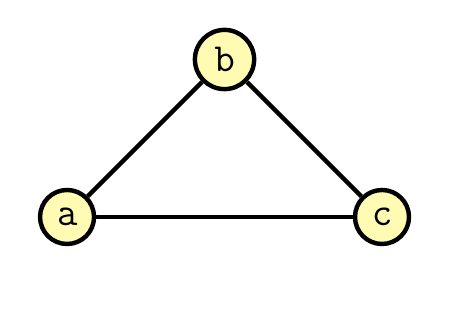
\begin{tikzpicture}[scale=1.00,transform shape]
\node[mynode] at (0.0, 0.0) (a) {a};
\node[mynode] at (2.0, 2.0) (b) {b};
\node[mynode] at (4.0, 0.0) (c) {c};
%
\draw[edgen] (a) edge node {} (b);
\draw[edgen] (b) edge node {} (c);
\draw[edgen] (c) edge node {} (a);

\path[use as bounding box] (-0.5,-1.00) rectangle (4.7, 2.0);
\end{tikzpicture}

\newpage

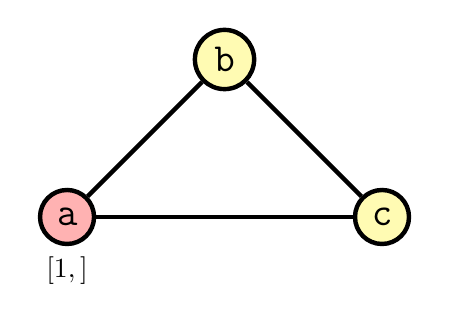
\begin{tikzpicture}[scale=1.00,transform shape]
\node[mynoder, label={below:$[1, ]$}] at (0.0, 0.0) (a) {a};
\node[mynode] at (2.0, 2.0) (b) {b};
\node[mynode] at (4.0, 0.0) (c) {c};
%
\draw[edgen] (a) edge node {} (b);
\draw[edgen] (b) edge node {} (c);
\draw[edgen] (c) edge node {} (a);

\path[use as bounding box] (-0.5,-1.00) rectangle (4.7, 2.0);
\end{tikzpicture}

\newpage

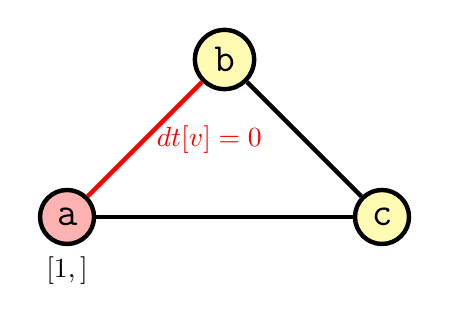
\begin{tikzpicture}[scale=1.00,transform shape]
\node[mynoder, label={below:$[1, ]$}] at (0.0, 0.0) (a) {a};
\node[mynode] at (2.0, 2.0) (b) {b};
\node[mynode] at (4.0, 0.0) (c) {c};
%
\draw[edger] (a) edge[right] node {$dt[v]=0$} (b);
\draw[edgen] (b) edge node {} (c);
\draw[edgen] (c) edge node {} (a);

\path[use as bounding box] (-0.5,-1.00) rectangle (4.7, 2.0);
\end{tikzpicture}

\newpage

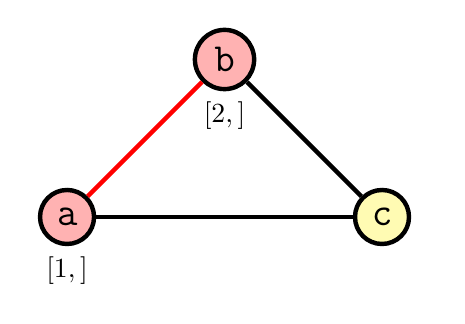
\begin{tikzpicture}[scale=1.00,transform shape]
\node[mynoder, label={below:$[1, ]$}] at (0.0, 0.0) (a) {a};
\node[mynoder, label={below:$[2, ]$}] at (2.0, 2.0) (b) {b};
\node[mynode] at (4.0, 0.0) (c) {c};
%
\draw[edger] (a) edge node {} (b);
\draw[edgen] (b) edge node {} (c);
\draw[edgen] (c) edge node {} (a);

\path[use as bounding box] (-0.5,-1.00) rectangle (4.7, 2.0);
\end{tikzpicture}

\newpage

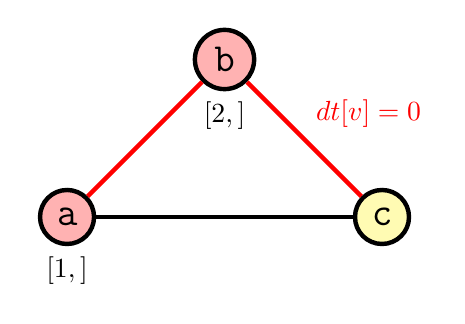
\begin{tikzpicture}[scale=1.00,transform shape]
\node[mynoder, label={below:$[1, ]$}] at (0.0, 0.0) (a) {a};
\node[mynoder, label={below:$[2, ]$}] at (2.0, 2.0) (b) {b};
\node[mynode] at (4.0, 0.0) (c) {c};
%
\draw[edger] (a) edge node {} (b);
\draw[edger] (b) edge[above right] node {$dt[v]=0$} (c);
\draw[edgen] (c) edge node {} (a);

\path[use as bounding box] (-0.5,-1.00) rectangle (4.7, 2.0);
\end{tikzpicture}

\newpage

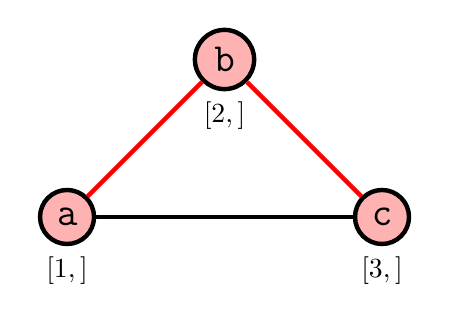
\begin{tikzpicture}[scale=1.00,transform shape]
\node[mynoder, label={below:$[1, ]$}] at (0.0, 0.0) (a) {a};
\node[mynoder, label={below:$[2, ]$}] at (2.0, 2.0) (b) {b};
\node[mynoder, label={below:$[3, ]$}] at (4.0, 0.0) (c) {c};
%
\draw[edger] (a) edge node {} (b);
\draw[edger] (b) edge node {} (c);
\draw[edgen] (c) edge node {} (a);

\path[use as bounding box] (-0.5,-1.00) rectangle (4.7, 2.0);
\end{tikzpicture}

\newpage

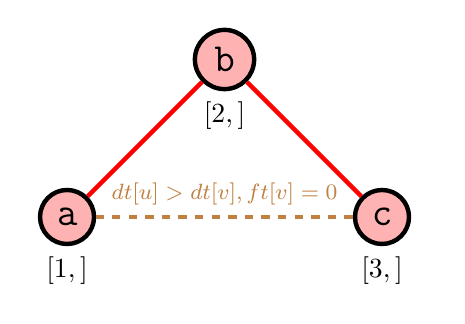
\begin{tikzpicture}[scale=1.00,transform shape]
\node[mynoder, label={below:$[1, ]$}] at (0.0, 0.0) (a) {a};
\node[mynoder, label={below:$[2, ]$}] at (2.0, 2.0) (b) {b};
\node[mynoder, label={below:$[3, ]$}] at (4.0, 0.0) (c) {c};
%
\draw[edger] (a) edge node {} (b);
\draw[edger] (b) edge node {} (c);
\draw[edgegd] (c) edge[above] node {\footnotesize $dt[u] > dt[v], ft[v] = 0$} (a); 

\path[use as bounding box] (-0.5,-1.00) rectangle (4.7, 2.0);
\end{tikzpicture}



\end{document}